\subsection{RQ1 --- How much does an explanation cost?}
\label{sec:rq1}
Table~\ref{tab:costfid} gives the cost and the quality of every explainer, and Fig.~\ref{fig:pareto} plots one against the other.

\begin{table}[!htbp]
\centering
\caption{Cost and quality of every explainer on the encrypted-traffic view $T_3$ (one CPU core). ms = median time per explanation; $\times$ = explanation time divided by the detector's own time; Faith.\ = faithfulness (higher is better); Infid.\ = infidelity (lower is better).}
\label{tab:costfid}
\scriptsize
\setlength{\tabcolsep}{3pt}
\begin{tabular}{llrrrr@{\hspace{10pt}}rrrr}
\toprule
 & & \multicolumn{4}{c}{\textbf{CIC-IDS2017}} & \multicolumn{4}{c}{\textbf{HIKARI-2021}} \\
\cmidrule(lr){3-6}\cmidrule(lr){7-10}
\textbf{Model} & \textbf{Explainer} & \textbf{ms} & $\boldsymbol{\times}$ & \textbf{Faith.} & \textbf{Infid.} & \textbf{ms} & $\boldsymbol{\times}$ & \textbf{Faith.} & \textbf{Infid.} \\
\midrule
LR & LinearSHAP & 0.006 & 0.1$\times$ & 0.44 & 0.80 & 0.006 & 0.1$\times$ & 0.15 & 0.95 \\
 & LIME-1000 & 23.19 & 302.5$\times$ & 0.39 & 0.83 & 22.40 & 322.8$\times$ & 0.44 & 0.68 \\
 & KernelSHAP-500 & 44.90 & 585.8$\times$ & 0.46 & 0.70 & 43.12 & 621.3$\times$ & 0.11 & 0.92 \\
\midrule
EBM & EBM-native & 0.33 & 0.8$\times$ & 0.47 & 0.75 & 0.30 & 0.8$\times$ & 0.70 & 0.14 \\
 & KernelSHAP-500 & 30.41 & 70.0$\times$ & 0.34 & 0.84 & 29.01 & 79.7$\times$ & 0.20 & 0.55 \\
\midrule
XGB & TreeSHAP-path & 0.98 & 1.8$\times$ & 0.60 & 0.59 & 1.23 & 3.2$\times$ & 0.46 & 0.65 \\
 & TreeSHAP-interv & 4.11 & 7.5$\times$ & 0.52 & 0.66 & 5.90 & 15.5$\times$ & 0.27 & 0.36 \\
 & LIME-500 & 19.34 & 35.4$\times$ & 0.28 & 0.81 & 21.57 & 56.7$\times$ & 0.17 & 0.41 \\
 & KernelSHAP-100 & 21.82 & 39.9$\times$ & 0.05 & 0.98 & 23.46 & 61.7$\times$ & 0.02 & 0.98 \\
 & LIME-1000 & 30.62 & 56.0$\times$ & 0.30 & 0.79 & 29.15 & 76.6$\times$ & 0.21 & 0.38 \\
 & LIME-5000 & 89.78 & 164.1$\times$ & 0.34 & 0.76 & 100.13 & 263.2$\times$ & 0.33 & 0.36 \\
 & KernelSHAP-500 & 109.39 & 200.0$\times$ & 0.49 & 0.68 & 99.13 & 260.5$\times$ & 0.23 & 0.41 \\
 & PartitionSHAP-500 & 174.06 & 318.2$\times$ & 0.28 & 0.78 & 176.59 & 464.1$\times$ & 0.29 & 0.42 \\
 & KernelSHAP-2048 & 374.10 & 684.0$\times$ & 0.50 & 0.67 & 390.83 & 1027.2$\times$ & 0.30 & 0.47 \\
\midrule
RF & TreeSHAP-path & 9.77 & 2.3$\times$ & 0.52 & 0.16 & 39.61 & 11.1$\times$ & 0.34 & 0.14 \\
 & TreeSHAP-interv & 13.62 & 3.2$\times$ & 0.60 & 0.16 & 37.40 & 10.5$\times$ & 0.23 & 0.06 \\
 & LIME-500 & 25.26 & 5.9$\times$ & 0.32 & 0.31 & 25.85 & 7.3$\times$ & 0.25 & 0.07 \\
 & KernelSHAP-100 & 33.20 & 7.7$\times$ & 0.07 & 0.95 & 35.37 & 9.9$\times$ & 0.03 & 1.00 \\
 & LIME-1000 & 35.53 & 8.3$\times$ & 0.32 & 0.32 & 34.98 & 9.8$\times$ & 0.27 & 0.09 \\
 & LIME-5000 & 106.73 & 24.9$\times$ & 0.33 & 0.34 & 102.59 & 28.8$\times$ & 0.29 & 0.23 \\
 & KernelSHAP-500 & 114.72 & 26.7$\times$ & 0.50 & 0.20 & 127.17 & 35.7$\times$ & 0.13 & 0.20 \\
 & KernelSHAP-2048 & 507.81 & 118.2$\times$ & 0.57 & 0.15 & 524.30 & 147.2$\times$ & 0.18 & 0.09 \\
\midrule
MLP & IG-16 & 1.13 & 14.9$\times$ & 0.56 & 0.62 & 1.03 & 17.2$\times$ & 0.45 & 0.50 \\
 & DeepSHAP & 1.56 & 20.6$\times$ & 0.30 & 0.85 & 1.84 & 30.7$\times$ & 0.09 & 0.94 \\
 & IG-32 & 1.62 & 21.3$\times$ & 0.56 & 0.60 & 1.64 & 27.3$\times$ & 0.45 & 0.51 \\
 & IG-64 & 2.89 & 38.1$\times$ & 0.55 & 0.62 & 2.90 & 48.4$\times$ & 0.45 & 0.51 \\
 & KernelSHAP-100 & 7.18 & 94.6$\times$ & 0.05 & 0.98 & 6.94 & 115.5$\times$ & 0.00 & 0.99 \\
 & LIME-500 & 17.80 & 234.5$\times$ & 0.27 & 0.87 & 16.45 & 273.9$\times$ & 0.24 & 0.76 \\
 & LIME-1000 & 23.27 & 306.5$\times$ & 0.28 & 0.88 & 22.52 & 375.1$\times$ & 0.25 & 0.75 \\
 & KernelSHAP-500 & 24.97 & 329.0$\times$ & 0.32 & 0.79 & 23.52 & 391.7$\times$ & 0.02 & 0.91 \\
 & LIME-5000 & 75.38 & 993.1$\times$ & 0.29 & 0.89 & 75.82 & 1262.6$\times$ & 0.25 & 0.76 \\
 & KernelSHAP-2048 & 91.94 & 1211.4$\times$ & 0.31 & 0.77 & 89.76 & 1494.7$\times$ & 0.04 & 0.92 \\
\bottomrule
\end{tabular}
\end{table}


\begin{itemize}[leftmargin=*, itemsep=0pt]
  \item \textbf{Two cost classes.} Model-specific explainers cost about as much as detection: the EBM's own explanations take 0.3\,ms, TreeSHAP on XGBoost about 1\,ms, and IG and DeepSHAP 1--3\,ms. Random Forest is the exception, because its large trees make TreeSHAP take 10--40\,ms. Model-agnostic explainers take 7--524\,ms: KernelSHAP grows with its sample budget, LIME needs 16--107\,ms and PartitionSHAP about 175\,ms.
  \item \textbf{Fewer features do not make explanations cheaper.} The 84-feature $T_1$ model costs about the same to explain as the 59-feature $T_3$ model (TreeSHAP 0.84 vs.\ 0.98\,ms).
  \item \textbf{Memory is not a problem} (at most 176\,MB), and timing is stable: for explainers above 5\,ms, the 99th percentile stays within 1.1--1.7 times the median.
  \item \textbf{H1 (at least 100$\times$ slower) is only partly true.} It holds for 25 of the 44 slow-explainer settings, up to 1{,}500$\times$. It fails on the slow Random Forest (7--37$\times$) and for small budgets, and with a fast explainer the time per flow grows only 1.1--49 times.
  \item \textbf{In flows per second:} on one core, XGBoost alone handles about 1{,}800 flows/s; with TreeSHAP for every flow it handles 660, and with KernelSHAP-500 only 9. Even if only the 5\% alerts are explained, KernelSHAP-500 limits a core to about 165 flows/s.
  \item \textbf{Paying more does not buy quality.} In 8 of 10 dataset--detector pairs the most faithful explainer is a fast model-specific one, usually 22--380 times cheaper than the best slow one. Across all settings, cost and faithfulness are not correlated ($\rho_s=-0.19$, $p=0.12$).
\end{itemize}

\begin{figure}[!htbp]
\centering
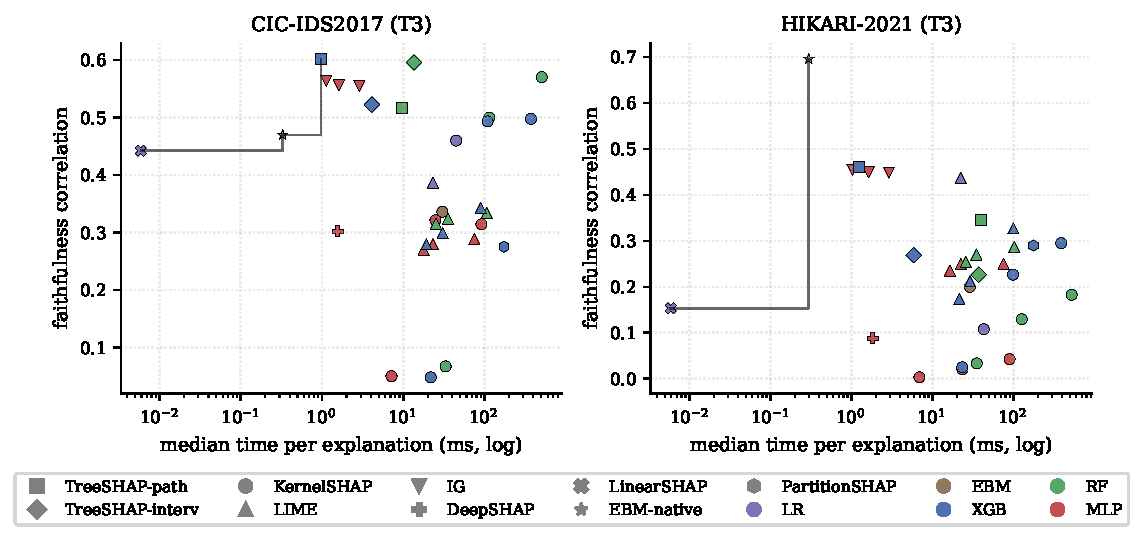
\includegraphics[width=0.9\textwidth]{../figures/fig_cost_fidelity_pareto.pdf}
\caption{Cost versus faithfulness of every explainer on $T_3$. The step line is the best trade-off (cheaper and more faithful is better).}
\label{fig:pareto}
\end{figure}
